\pandocbounded{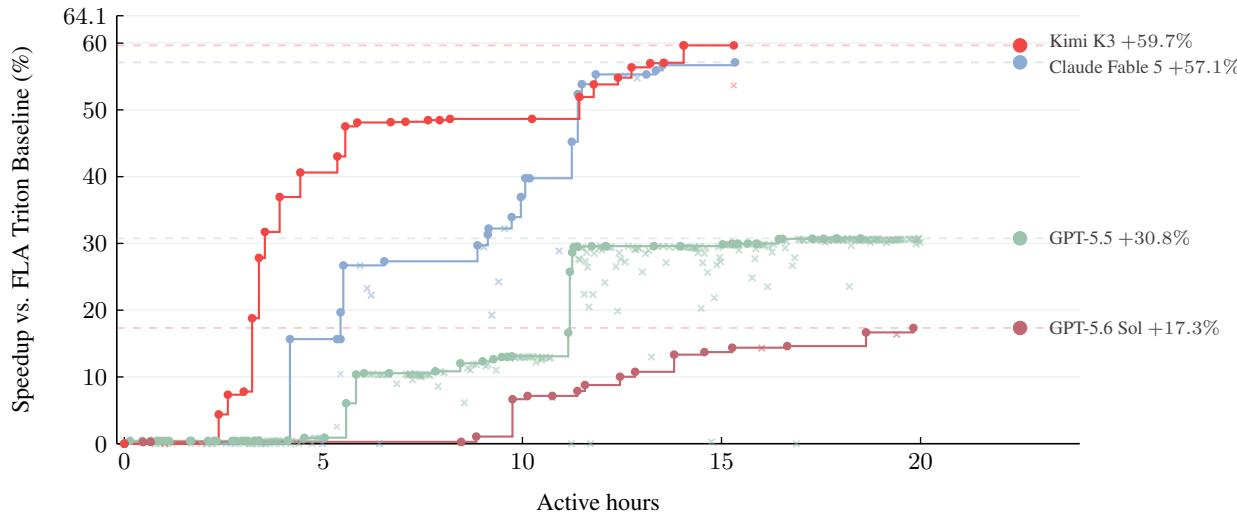
\includegraphics[keepaspectratio,alt={image}]{images/fe44c03c3b161a2550b601fadb4b5bdf3ad4855a9eabcdd3f269b72ee50b15b7.jpg}}

图 14: 案例研究：AttnRes 上的 GPU 内核优化。

\section{案例研究}\label{case-studies}

在本节中，我们展示代表 Kimi K3 在多种技术任务中能力的典型案例。

GPU 内核优化 我们测试了模型优化 GPU 内核的能力。每个模型在相同配置的沙箱中独立工作，每个任务最多有 24 小时的预算用于性能分析、重写和基准测试。评估涵盖四个代表性内核：AttnRes、DeepSeek Sparse Attention (DSA)、KDA 和 MLA（头维度 512），运行在 NVIDIA Hopper GPU 和一款替代供应商的 GPGPU 上。Kimi K3 在所有四个内核上都实现了显著性能提升：将 AttnRes 延迟从 283.6 ms 降至 114.4 ms，将 DSA 和 KDA 运行时间分别缩短 55.1\% 和 73.6\%，并在 MLA 上达到峰值 TFLOPS 的一半以上。在这些任务中，Kimi K3 匹敌 Claude Fable 5 {[}16{]}（含回退）并显著优于 Claude Opus 4.8 {[}17{]}、GPT-5.6 Sol {[}39{]} 和 GPT-5.5 {[}38{]}。图 14 比较了各模型在 AttnRes 上的优化轨迹。除了基准测试之外，在开发后期，Kimi K3 的早期检查点已经承担了我们大部分的内核优化工作。

GPU 编译器开发 Kimi K3 开发了 MiniTriton5，一个紧凑的类 Triton {[}122{]} 编译器，包含自定义的 tile 级 Python 前端和布局系统、轻量级的 warp 级 MLIR {[}64{]} 标注与优化层，以及 Parallel Thread Execution (PTX) 代码生成流水线。编译器之上构建了一个双模式张量库，提供类 PyTorch {[}89{]} 的高层接口，其 eager 和前向编译路径共享相同的 DSL 编译器和运行时。该库进一步提供反向模式 autograd、神经网络模块、基于 NCCL {[}82{]} 的分布式训练原语，以及稀疏和可视化原语。在 NVIDIA L20 上，MiniTriton 在其核心基准套件的几何平均上优于 PyTorch eager {[}89{]} 和 torch.compile {[}5{]}。其从零实现的 tensor-core matmul 路径在大尺寸上接近 cuBLAS {[}22{]}，达到约 90\% 的实测机器性能上限；而其 DSL 级别的 KDA {[}63{]} prefill 内核以明显优势优于匹配的 Triton 参考实现。MiniTriton 还端到端训练了一个 GPT 模型，其损失曲线与 PyTorch 参考实现紧密跟踪，全模型梯度与 torch autograd 的差异不超过 torch 自身 fp32 舍入误差（10^{-4}，以 fp64 参考为基准）。总的来说，这些结果表明 Kimi K3 能够构建一个连贯的端到端编译器——从 DSL 前端和 IR 遍到 PTX 代码生成和 CUDA 运行时——而不仅仅是一组孤立的内核（图 15）。

芯片设计 作为早期概念验证，Kimi K3 为一个 nano 模型设计了推理芯片原型，该模型遵循相同的架构——混合 KDA 和 NoPE-MLA 注意力、块大小为 2 的 Block AttnRes、基于 sigmoid 的 MoE 路由（含一个共享专家）——采用分组 INT4 权重量化（组大小 128）。在一次 48 小时的 Kimi Code 自主运行中，Kimi K3 使用开源 EDA 工具和 Nangate45 标准单元库 {[}80{]} 构建、优化并验证了该芯片。在 4 mm² 的分析面积预算内，该设计在 100 MHz 频率下满足时序要求，并实现 RTL 仿真解码吞吐量超过 8,700 tokens/s，集成了 146 万标准单元、0.277 MiB SRAM 和一个带融合反量化的 INT4 MAC 阵列。RTL 代码可在 GitHub6 上获取。

MiniTriton CUDA-core roofline --- NVIDIA L20 (sm\_89), fp32

\pandocbounded{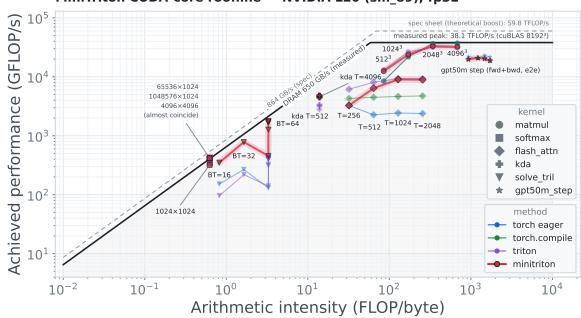
\includegraphics[keepaspectratio,alt={image}]{images/dc011552c6aebfbfda90bba8a0e54ea6ca6195095b859fa831fe8d0bc8177626.jpg}}

MiniTriton tensor-core roofline --- NVIDIA L20 (sm\_89)

\pandocbounded{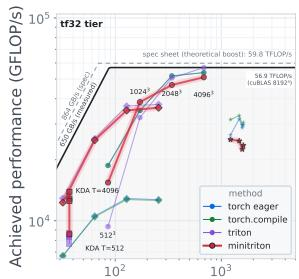
\includegraphics[keepaspectratio,alt={image}]{images/2cd2bd6535e57155908473d8e47322fc2fb15db717e329a05cc0c2bc53601d83.jpg}}

\pandocbounded{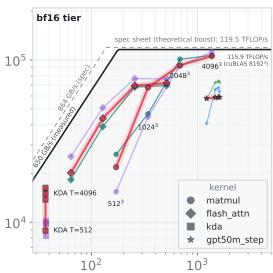
\includegraphics[keepaspectratio,alt={image}]{images/2690b67cf77b170aa823b51977a867441378a7a7ae97ad5dc32e6bb95c509f56.jpg}}

算术强度 (FLOP/byte) 算术强度 (FLOP/byte)

\begin{enumerate}
\def\labelenumi{(\alph{enumi})}
\tightlist
\item
  CUDA-core roofline, fp32
\end{enumerate}

train\_gpt 收敛 --- minitriton vs torch eager

\pandocbounded{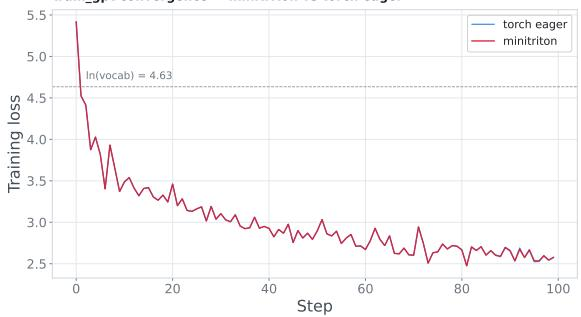
\includegraphics[keepaspectratio,alt={image}]{images/abaf0bdd61e59519fd738dcc9ed14a6fa016dbcfd97b6236ce5fb9046912cd3e.jpg}}

\begin{enumerate}
\def\labelenumi{(\alph{enumi})}
\setcounter{enumi}{2}
\item
  收敛性 vs.~torch eager
\item
  Tensor-core rooflines, tf32/bf16
\end{enumerate}

\pandocbounded{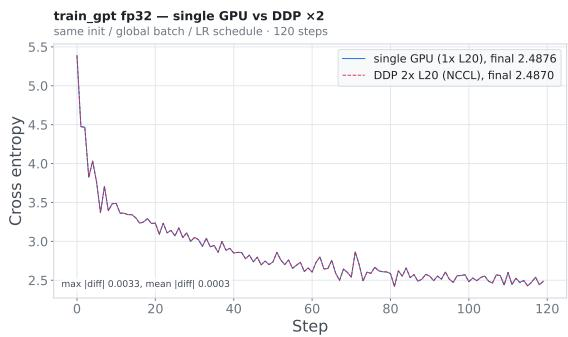
\includegraphics[keepaspectratio,alt={image}]{images/56ade52ffc9804a868ec6588558809e819f0882aa3925e7fe799c33e8cdebf04.jpg}}

\begin{enumerate}
\def\labelenumi{(\alph{enumi})}
\setcounter{enumi}{3}
\tightlist
\item
  双 GPU DDP vs.~单 GPU
\end{enumerate}

图 15: 案例研究：基于 MiniTriton 的 GPU 编译器开发。(a) MiniTriton 内核在 NVIDIA L20 (sm\_89) 上的 CUDA-core 和 (b) tensor-core roofline，对比 torch eager、torch.compile、Triton 和 cuBLAS 基线（含未达标点）；(c) 使用 MiniTriton 与 torch eager 训练的字符级 GPT 的训练损失曲线；(d) 基于 MiniTriton 自有分布式原语（NCCL）的双 GPU 数据并行训练与单 GPU 训练的对比。

科研编程 为复现计算天体物理中的 I-Love-Q 普适关系，Kimi K3 审阅了超过 20 篇论文并交叉验证其结果，实现了完整的数值流水线，评估了超过 300 个状态方程，识别了已发表公式中的不一致之处，编写了超过 3,000 行 Python 代码，并生成了一个交互式 HTML 仪表盘——耗时约两小时，而一位经验丰富的研究者通常需要一到两周。

知识工作 在 Kimi Work 中，Kimi K3 制作了一个覆盖 AI ASIC 行业 42 年历史的交互式研究网站。该模型完成了超过 120 轮迭代优化，依托 87 份季度报告和 99 份原始 PDF（超过 11,000 页）的语料，通过超过 2,800 次网页搜索和超过 1,100 次终端查询完成。在另一个案例中，Kimi K3 使用超过 20 个并发子代理分析了 GWTC-5 中的 391 个引力波事件，生成了七个科学可视化、两个汇总表和超过十篇论文的文献综述。

视频剪辑与动态设计 利用其原生多模态架构，Kimi K3 创建了一个 3Blue1Brown 风格的动态图形解说视频来介绍其自身架构，并从 56 个源片段中剪辑了其预告片。这涉及片段选择、动匹配剪辑、逐帧节拍同步、音频处理以及多轮修改。制作一段类似水准的高密度短视频通常需要一位经验丰富的剪辑师一到两天。

\section{结论}\label{conclusion}

我们提出了 Kimi K3，一个开放的 2.8 万亿参数混合专家模型，具备原生视觉能力和 100 万 token 上下文窗口，基于 Kimi Delta Attention 和 Attention Residuals 构建。作为全球首个开放的三万亿级模型，Kimi K3 在长周期编程、智能体、知识、推理和视觉任务中展现了前沿级性能。尽管与最强闭源模型之间仍存在差距，但 Kimi K3 在每个人都触手可及的范围内建立了一个新的开放前沿。我们希望它能赋能更广泛的社区进行研究、部署和创新。
